\documentclass[12pt]{article} 
\usepackage[utf8]{inputenc}
\usepackage{geometry}
\geometry{letterpaper}
\usepackage{graphicx} 
\usepackage{parskip}
\usepackage{booktabs}
\usepackage{array} 
\usepackage{paralist} 
\usepackage{verbatim}
\usepackage{subfig}
\usepackage{fancyhdr}
\usepackage{sectsty}
\usepackage{enumitem}

\pagestyle{fancy}
\renewcommand{\headrulewidth}{0pt} 
\lhead{}\chead{}\rhead{}
\lfoot{}\cfoot{\thepage}\rfoot{}


%%% ToC (table of contents) APPEARANCE
\usepackage[nottoc,notlof,notlot]{tocbibind} 
\usepackage[titles,subfigure]{tocloft}
\renewcommand{\cftsecfont}{\rmfamily\mdseries\upshape}
\renewcommand{\cftsecpagefont}{\rmfamily\mdseries\upshape} %

\usepackage{amsmath}
\usepackage{amssymb}
\usepackage{mathtools}
\usepackage{empheq}
\usepackage{xcolor}

\usepackage{tikz}
\usepackage{pgfplots}
\pgfplotsset{compat=1.18}

\newcommand{\ans}[1]{\boxed{\text{#1}}}
\newcommand{\vecs}[1]{\langle #1\rangle}
\renewcommand{\hat}[1]{\widehat{#1}}
\newcommand{\F}[1]{\mathcal{F}(#1)}
\renewcommand{\P}{\mathbb{P}}
\newcommand{\R}{\mathbb{R}}

\newcommand{\E}{\mathbb{E}}
\newcommand{\Z}{\mathbb{Z}}
\newcommand{\ind}{\mathbbm{1}}
\newcommand{\qed}{\quad \blacksquare}
\newcommand{\brak}[1]{\langle #1 \rangle}
\newcommand{\bra}[1]{\langle #1 |}
\newcommand{\ket}[1]{| #1 \rangle}

\title{Math 1530: Homework 2}
\author{Milan Capoor}
\date{26 September 2023}

\begin{document}
\maketitle
\section*{2.26}
\emph{Let $G$ be a group and let $g\in G$ be an element of order $n$, and let $k \geq 1$.} 

\begin{enumerate}[label=(\alph*)]
    \item \emph{Prove that $g^k$ has order $n/\gcd(n, k)$}

    \color{blue}
        Because $G$ has an element of order $n$, we know that 
        \[(g^k)^{\frac{n}{\gcd(n, k)}} = (g^n)^{\frac{k}{\gcd(n, k)}} = e\]
        so 
        \[o(g^k) \bigg\vert \frac{n}{\gcd(n, k)}\]
        Now to show that this quantity is the order of $g^k$, we just need to show that it is the smallest value for which the above is true, 

        We choose an $m$ that satisfies
        \[(g^k)^{m} = g^{km} = e\]
        So 
        \[n | km \implies \frac{n}{\gcd(k, n)} \bigg\vert \frac{km}{\gcd(k, n)}\]
        However, 
        \[\gcd\left(\frac{n}{\gcd(k, n)}, \frac{k}{\gcd(k, n)}\right) = 1\]
        (Because if they were not relatively prime, there would be a bigger $\gcd(k, n)$)
        So
        \[\frac{n}{\gcd(k,n)} \bigg \vert m \implies \frac{n}{\gcd(k,n)} \leq m\]
        Which shows that for any $m$ which satisfies the equation, it is still greater than or equal to $\frac{n}{\gcd(k,n)}$. Hence, $o(g^k) = \frac{n}{\gcd(k,n)} \qed$

    \color{black}

    \item \emph{Use (a) to give a quick proof that if $G = \brak{g}$ is a cyclic group of order $n$, then $g^k$ generates $G$ iff $\gcd(n,k)= 1$}
    
    \color{blue}
        Since $G$ is a group of order $n$, $g^k$ can only be a generator if
        \[o(g^k) = o(G) = n\]
        But from (a), 
        \[o(g^k) = \frac{n}{\gcd(k,n)} \implies \frac{n}{\gcd(k,n)} = n \implies \gcd(k,n) = 1 \qed\]
    \color{black}
\end{enumerate}
\pagebreak 

\section*{2.28}
\emph{Let $G$ be a group and let $H \subset G$ be a subset of $G$. Prove that $H$ is a subgroup iff it has the following two properties:}
\begin{enumerate}
    \item $H \neq \emptyset$
    \item \emph{For every $h_1, h_2 \in H$, the product $h_1 \cdot h_2^{-1}$ is in H.}
\end{enumerate}

\color{blue}
    To be a subgroup, $H$ must satisfy the properties of a group. Namely, it must have an identity and inverse element. Clearly, if $H = \emptyset$ it has neither so it would not be a subgroup. 

    Then, if with $h_1 = h_2$, the element $h_1 h_2^{-1} = h_1 h_1^{-1} = e$ were not in $H$, the set would not have an identity element and would not be a group.

    Similarly, let $h_1 = e$. Then, if the element $h_1 h_2^{-1} = h_2^{-1}$ is not in $H$, then not every $h_2$ would have an inverse element $h_2^{-1}$ and $H$ would not be a group. Letting $h_2 = e$ identically shows that the inverse of every $h_1$ must be in the set. 

    By these contradictions, then, both properties must be true for $H$ to be a subgroup of $G. \qed$
\color{black}
\pagebreak

\section*{2.30}
Let $G$ be a group and let $S \subseteq G$ be a subset of $G$. 
\[\brak{S} = \bigcap_{S \subseteq H \subset G} H\]
\emph{i.e., $\brak{S}$ is the intersection of all subgroups $H$ of $G$ that contain $S$}

\begin{enumerate}[label=(\alph*)]
    \item \emph{Prove that $\brak{S} \neq \emptyset$}
    
    \color{blue}
        All the subgroups $H$ must contain the identity element so, at minimum,
        \[\brak{S} = \bigcap H = \{e\} \neq \emptyset \qed\]
    \color{black}
    
    \item \emph{Prove that $\brak{S}$ is a subgroup of $G$. }
    
    \color{blue}
        From above, $\brak{S}$ has an identity. Additionally, all subgroups of $H \subseteq G$ have an inverse for every $h \in H$ by definition. As $\brak{S}$ is defined as the intersection of the subgroups $H$, every element in the intersection thus must also has an inverse in the intersection, so every $s \in \brak{S}$ has an inverse. Therefore, $\brak{S}$ satisfies the identity and inverse requirements and is a subgroup. $\qed$
    \color{black}

    \item \emph{Suppose that $K \subseteq G$ is a subgroup of $G$ and that $S \subseteq K$. Prove that $\brak{S} \subset K$. ($\brak{S}$ is the smallest subgroup of $G$ that contains $S$.)}
    
    \color{blue}
        If $S \subset K$, then by definition of $\brak{S}$, 
        \[\brak{S} = K \cap \left(\underset{H\neq K}{\bigcap_{S \subseteq H \subset G}} H\right)\]
        However, by the properties of intersection, 
        \[A \cap B \subseteq A \quad \forall B\]
        so 
        \[K \cap \left(\underset{H\neq K}{\bigcap_{S \subseteq H \subset G}} H\right) \subseteq K \implies \brak{S} \subseteq K \qed\]
    \color{black}

    \item \emph{Let $T$ be the set of inverses of elements in $S$, }
    \[T = \{g^{-1} : g \in S\}\]
    \emph{Prove that $\brak{S}$ is equal to the following set of products:}
    \[\brak{S} = \{g_1 g_2 \dots g_n : n \geq 0 \text{ and } g_1, \; \dots, g_n \in S \cup T\}\]

    \color{blue}
        Because the product $g_1 g_2 \dots g_n$ is defined for all $n \geq 0$, every element $g_i \in S$ is in $S \cup T$ (Let $g_1 = g_i$ and $n = 1$) and so is $g_i^{-1}$ ($g_1 = g_i^{-1}$). The identity corresponds to $n=0$. Thus $H = \left\{\prod_{i=1}^n g_n\right\}$ is a subgroup of $G$. 
        
        Because every element $g_i$ is either in $S$ or is the inverse of an element in $S$, removing any element from $H$ means that either there will be an element of $S$ that is not in $H$ or $H$ will not be a group. Thus, $H$ is the smallest subgroup of $G$ that contains all of $S$. But from part (c), $\brak{S}$ is the smallest subgroup of $G$ that contains $S$ so 
       \[\brak{S} = \{g_1 g_2 \dots g_n : n \geq 0 \text{ and } g_1, \; \dots, g_n \in S \cup T\} \qed\]
    \color{black}
\end{enumerate}
\pagebreak

\section*{2.35}
\emph{Let $G$ be a group. The center of $G$ denoted $Z(G)$ is the set of elements of $G$ that commute with every other element:}
\[Z(G) = \{g \in G: gh = hg \; \forall h \in G\}\]

\begin{enumerate}[label=(\alph*)]
    \item \emph{Prove that $Z(G)$ is a subgroup of $G$}
    
    \color{blue}
        By definition, the identity element $e$ of $G$ satisfies $eh = he = h$ for all $h \in G$. Similarly, the inverse $h^{-1}$ is defined as the element which satisfies $hh^{-1} = h^{-1}h = e$ for all $h$ is $G$. Thus, as they are commutative with all elements of $G$, both the inverse and identity of $G$ are in $Z(G)$, so $Z(G)$ is a group. $\qed$
    \color{black}

    \item \emph{When does $Z(G)$ equal $G$ }
    
    \color{blue}
        When $G$ is an abelian group.
    \color{black}

    \item \emph{Compute the center of the symmetric group $\mathcal{S}_n$}
    
    \color{blue}
        For $n = 1$, the center is obviously the entire group. For $n = 2$, the two elements are the identity which is commutative (and so in the center) for all groups and the reversal of the elements which is its own inverse and is thus also in the center.

        For $n \geq 3$, let $\sigma \in S_n: \sigma \neq e$ and let $i, j, k$ be distinct values in $\{1, 2,\; \dots, n\}$. Let $\sigma(i) = j$ and $\sigma(j) = k$. Note that $\sigma$ is an arbitrary permutation of $\{1, 2,\; \dots, n\}$. Now consider 
        \[\tau(x) = \begin{cases}
            j \quad x = i\\
            i \quad x = j\\
            x \quad \text{otherwise}
        \end{cases}\]

        Thus,
        \begin{align*}
            (\tau \circ \sigma)(i) &= \tau(j) = i\\
            (\sigma \circ \tau)(i) &= \sigma(j) = k\\
            i \neq j &\implies (\tau \circ \sigma)(i) \neq (\sigma \circ \tau)(i)
        \end{align*}
        So we have found an element in $S_n$ which $\sigma$ does not commute with. But because $\sigma$ is any arbitrary permutation ($\sigma \neq e$), then there is no element in $S_{n\geq 3}$ which commutes with every element so the center of $S_n$ is $\{e\} \qed$.  
    \color{black}
    
    \item \emph{Compute the center of the dihedral group $\mathcal{D}_n$}
    
    \color{blue}
        Let $P$ be a $2n$-gon. Let $a$ be a reflection. Label the vertices of $P$ by ${0, 1, \; \dots \; 2n - 1}$. 
        
        Let $a$ be a flip such that $a(0) = 0$, $a(n) = n$, and all the other vertices are moved counterclockwise (i.e. $a(1) = 2n -1$). Let $b$ be the clockwise rotation $b(0) = 1, b(1) = 2, \dots$.

        For $n=3$, for example, the two transformations can be represented:
        \begin{center}
            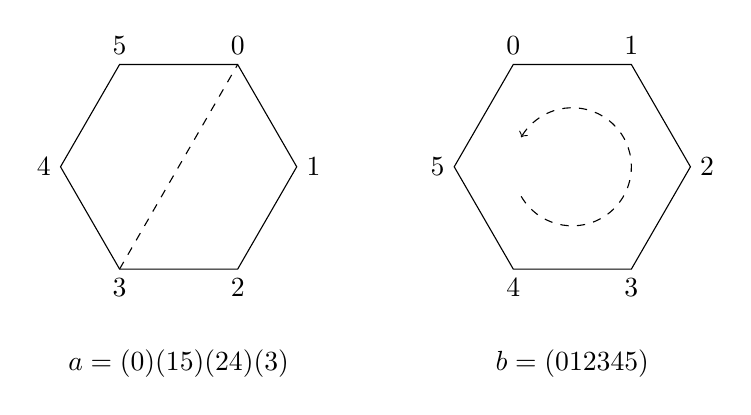
\begin{tikzpicture}
                \newdimen\R
                \R=1.5cm
                \draw (0:\R)
                    \foreach \x in {60,120,...,360} {  -- (\x:\R) }
                        -- cycle (360:\R) node[right] {1}
                        -- cycle (300:\R) node[below] {2}
                        -- cycle (240:\R) node[below] {3}
                        -- cycle (180:\R) node[left] {4}
                        -- cycle  (120:\R) node[above] {5}
                        -- cycle  (60:\R) node[above] {0};
                \draw[dashed] (240:\R) -- (60:\R);
                \node[yshift=-2.5cm]{$a = (0)(15)(24)(3)$};
                
                \draw[xshift=5cm] (0:\R)
                \foreach \x in {60,120,...,360} {  -- (\x:\R) }
                    -- cycle (360:\R) node[right] {2}
                    -- cycle (300:\R) node[below] {3}
                    -- cycle (240:\R) node[below] {4}
                    -- cycle (180:\R) node[left] {5}
                    -- cycle  (120:\R) node[above] {0}
                    -- cycle  (60:\R) node[above] {1};
                \draw[dashed, xshift=5cm, ->] (-150:{0.5*\R}) arc (-150:150:{0.5*\R});
                \node[yshift=-2.5cm, xshift=5cm]{$b = (012345)$};
            \end{tikzpicture}
        \end{center}
        
        Then 
        \begin{align*}
            (a \circ b)(0) &= a(1) = 2n-1\\
            (b \circ a)(0) &= b(0) = 1\\
            1 \neq 2n - 1 &\implies ab \neq ba
        \end{align*}
        But as $a$ is an arbitrary reflection that can be transformed into any other reflection through a re-labeling of vertices or a rotation of the entire system, we can conclude that no reflections are commutative with every element of $D_{2n}$ (because we have a counter example) so no reflection is part of the center of $D_{2n}$. 
        
        For odd n-gons we can make exactly the same argument but with $a$ satisfying only $a(0) = 0$, $a(1) = n - 1$. Using the same $b$, 
        \begin{align*}
            (a \circ b)(0) &= a(1) = n - 1\\
            (b \circ a)(0) &= b(0) = 1\\
            1 \neq n - 1 &\implies ab \neq ba
        \end{align*}
        So reflections are not in the center of any dihedral group. 

        Now, all that remains is to classify the rotations. Notice, however, that reversing the argument given above shows that a rotation by $\frac{2\pi}{n}$ radians (for an n-gon) does not commute with any reflection so it cannot be in the center. Are any of the composite rotations $r^m = \frac{2\pi}{n}m \quad (m \leq n)$ in $Z(D_n)$? 

        First we observe that all reflections are commutative with each other because $\brak{r}$ is an abelian subgroup. Then we notice that the composition of a clockwise rotation and a flip results in a net counterclockwise rotation (the order of $\brak{r} = n$ so every vertex is can be permuted to every other vertex by rotations) and vice versa. Meanwhile, the composition of a flip and a rotation preserves the direction of the rotation. Thus, the only way that the two compositions could commute were if a clockwise and counterclockwise rotation resulted in the same point. For odd n-gons the only rotation with this property is the identity. For even n-gons, a rotation by $\pi$ radians (i.e. when $m = \frac{n}{2}$) satisfies the property $r^{\frac{n}{2}} = r^{\frac{-n}{2}}$. Thus the only rotation that can commute with any reflection is the rotation by $\pi$ radians for n-gons of even $n$. Then because all rotations commute, the rotation $r^{n/2}$ commutes with every element of $D_n$. 
        
        Thus, the only elements in $Z(D_n)$ are $\{e\}$ and $r^{n/2}$ (for n-gons of even $n$). $\qed$
    \color{black}

    \item \emph{Compute the center of the quaternion group $\mathcal{Q}$}
    
    \color{blue}
        \[\mathcal{Q} = \{\pm 1, \pm i, \pm j, \pm k\}\] 
        From Exercise 2.17, 
        \begin{align*}
            {i \cdot j} &= k, &{j \cdot k} &= i,&{k \cdot i} &= j\\
            {j \cdot i} &= -k, & {k \cdot j} &= -i, & {i \cdot k} &= -j
        \end{align*}
        So none of the compositions of $i, j, k$ are commutative so the only operations in the center are $\boxed{\{1, -1\}}$
    \color{black}
\end{enumerate}
\pagebreak

\section*{2.38}
\emph{Let $G$ be a finite group whose only subgroups are $\{e\}$ and $G$. Prove that either $G = \{e\}$ or else that $G$ is a cyclic group with prime order.}

\color{blue}
    If $G = \{e\}$, we are done. Otherwise, it has an element $g$ and a subgroup $H = \brak{g}$. However, because we know that the only subgroups of $G$ are $\{e\}$ and $G$, $H= \{e\}$ or $H = G$. If $H = \{e\}$ then the only element is $e$ which is a contradiction so $H =\brak{g} = G$. Thus, $g$ is a generator of $G$ so $G$ is cyclic with order $o(g)$. 

    $o(g)$ can either be composite or prime. Assume it is composite. Then $o(g)$ has a prime factorization, i.e. there are at least two primes $p, q$ for which $p^n | o(g)$ and $q^m | o(g)$ for some $m$ and $n$. By Sylow's theorem, $G$ thus has subgroups of order $p^n$ and $q^m$. But this contradicts the fact that $G$ only has two subgroups. Thus $o(g)$ can only have one prime factor $p^n = o(g)$. Further, we can use a similar argument to show that if $p^n = o(g)$, $p | o(g)$ so $G$ must have a subgroup with order $p$ but its only subgroup is order $o(g)$ so $n =1$ and $p = o(g)$. 
    
    Hence, $o(g)$ must be a cyclic group of prime order. $\qed$
\color{black}
\end{document}